\chapter{Program Stubs and Test Data Required}
\label{chap:stubs}

In order to perform integration testing without having developed first the entire system (``big bang'' approach) we need to use stubs and drivers to take the part of the software components that still don't exist and test the others.

\begin{description}
    \item[Test database:] the testing environment must include a DBMS configured in the same way of the production. The test data contained in this database includes a reduced set of instances of all the entities described in the Entity-Relation diagram of the Design Document~\cite[p.~10]{mytaxi-dd}, which is reported in~\autoref{fig:er-diagram}

    \item[Lightweight API client:] in order to sest the REST API of the business tier without the actual client application, a simple API client which interacts with the business tier by simple HTTP requests is needed. This driver needs to be scriptable in order for the tests to be automated.

    \item[Drivers for the Java Entity Beans:] they are used to test the Java Entity Beans when the Business Tier is not fully developed. They call the relevant methods of the EJBs to test the correctness of the queries.

    \item[Stub of the Business Tier:] used to provide a minimum set of data to test the web tier when the business tier is not fully developed.
\end{description}
%TODO to complete

\begin{figure}
    \centering
    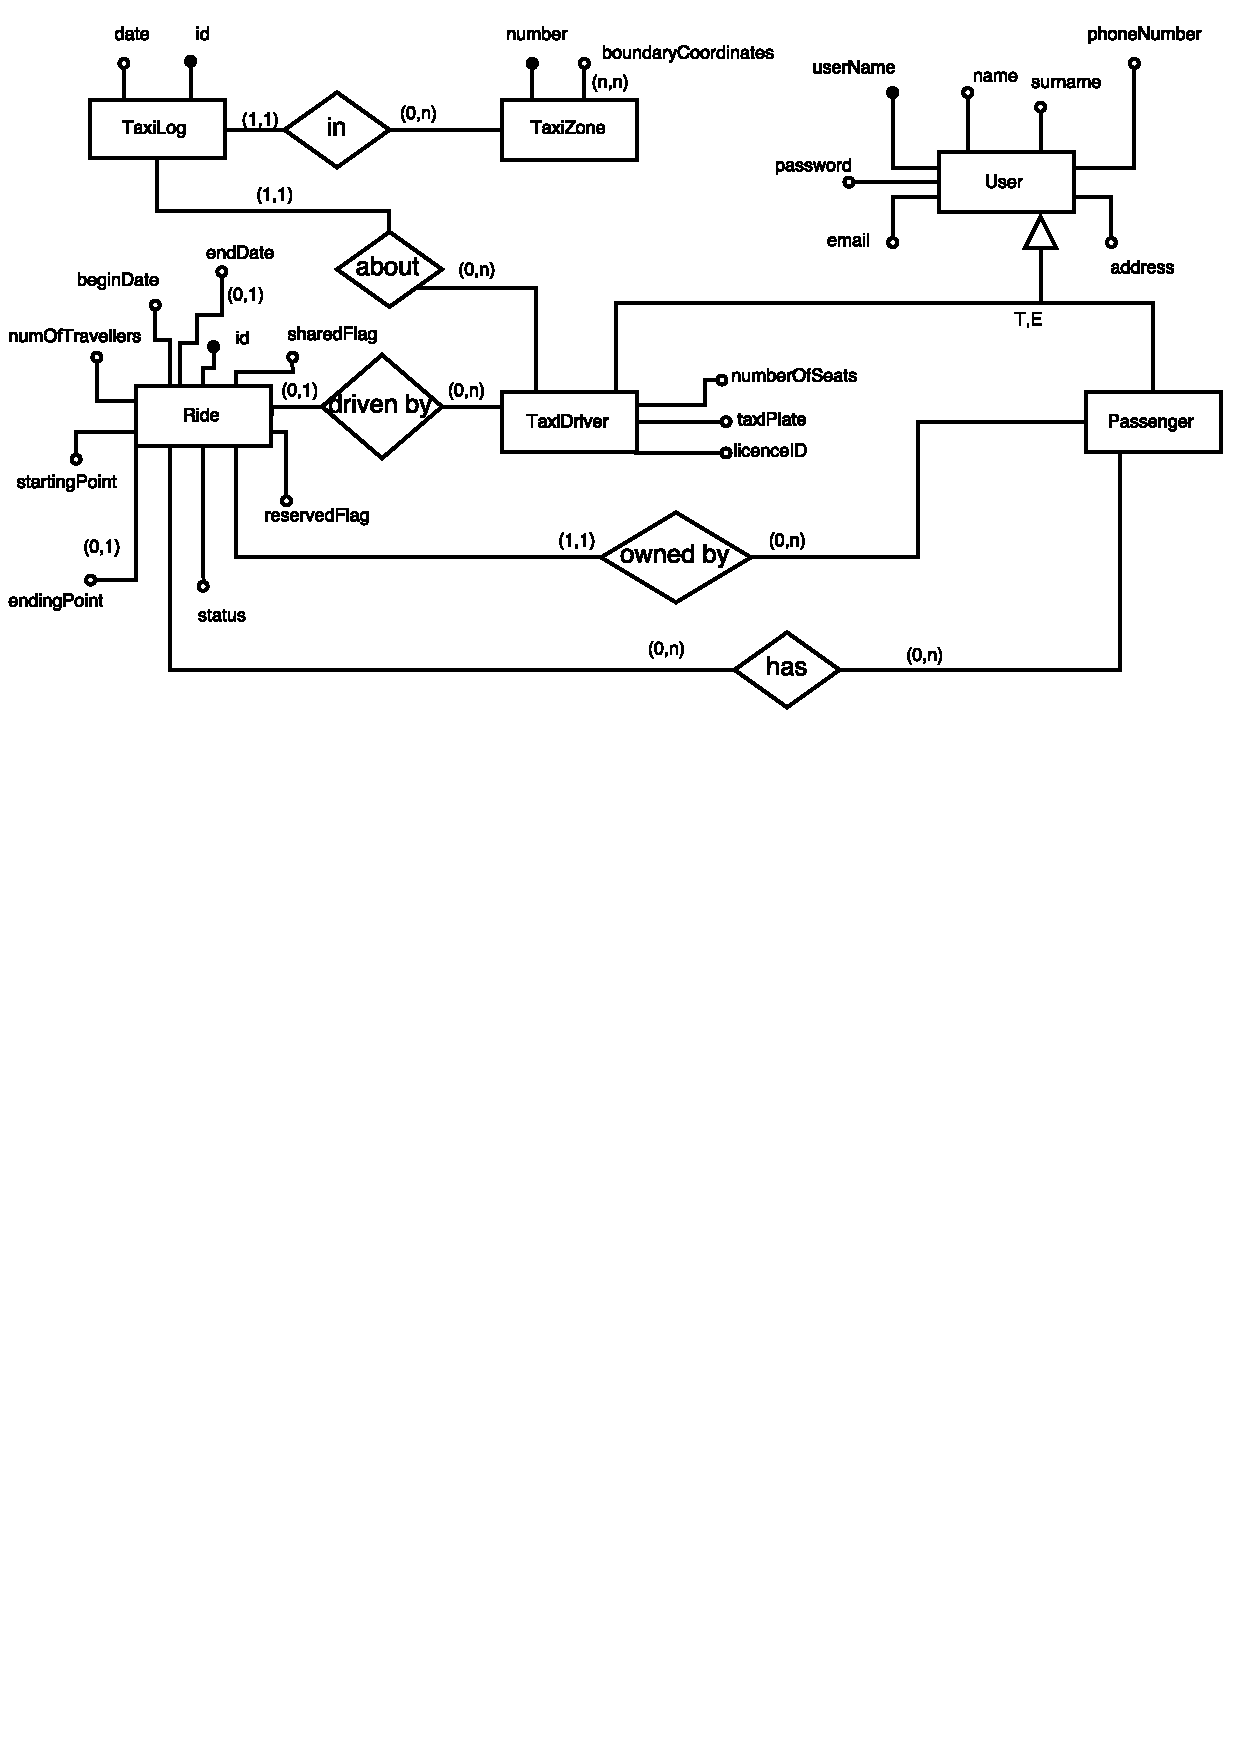
\includegraphics[width=\textwidth]{../dd/diagrams/er_diagram.pdf}
    \caption{ER diagram of the database schema as specified in the Design Document~\cite{mytaxi-dd}.}
    \label{fig:er-diagram}
\end{figure}
